\documentclass[12pt,a4paper]{article}
\usepackage[latin1]{inputenc}
\usepackage{amsmath}
\usepackage{amsfonts}
\usepackage{amssymb}
\usepackage{graphicx}

\newcommand{\la}{\lambda}
\newcommand{\La}{\Lambda}
\newcommand{\al}{\alpha}
\newcommand{\si}{\sigma}
\newcommand{\Si}{\Sigma}
\newcommand{\ga}{\gamma}
\newcommand{\Ga}{\Gamma}
\newcommand{\be}{\beta}
\newcommand{\te}{\theta}
\newcommand{\de}{\delta}
\newcommand{\De}{\Delta}
\newcommand{\pr}{\prime}
\newcommand{\mbf}{\mathbf}


\newcommand{\pas}{\partial}
\newcommand{\mbb}{\mathbb}
\newcommand{\mc}{\mathcal}
\newcommand{\mf}{\mathfrak}
\newcommand{\mi}{\mathit}
\newcommand{\ms}[1]{\mathsf{#1}}
\newcommand{\na}{\nabla}
\newcommand{\nonb}{\nonumber}
%######################################################################
\newcommand{\D}{\mathbb{D}}
\newcommand{\Z}{\mathbb{Z}}
\newcommand{\Q}{\mathbb{Q}}
\newcommand{\R}{\mathbb{R}}
\newcommand{\C}{\mathbb{C}}
\newcommand{\N}{\mathbb{N}}
\newcommand{\F}{\mathbb{F}}
\newcommand{\K}{\mathbb{K}}
\newcommand{\E}{\mathcal{E}}

   


\begin{document}
			\begin{center}
		UNIVERSITE D'ABOMEY CALAVI (UAC) 	\\
	\end{center}
	
	\begin{center}
		INSTITUT DE MATHEMATIQUE ET DE SCIENCES PHYSIQUES (IMSP)     	\\
	\end{center}
	\begin{center}
		Centre d'Excellence Africain en Science Math�matiques et Applications: (CEA-SMA)\\
		\vspace{1cm}
		Master 1 Math�matiques fondamentales\\
	\end{center}
	\vspace{1.5cm}
	\begin{center} 
 $\scalebox{2}{ Projet d'Optimisation num�rique }$ \\
 	\vspace{1cm}
      
  Optimisation du profil d'une route\\
 
	\end{center}
	\vspace{9cm}
	Pr�sent� par:   \hfill Supervis� par :\\
	Anne-Marie AHOUNOU   \hfill Professeur Marie POSTEL \\
	Kenneth ASSOGBA\\\\
	
%\begin{enumerae}
\section*{Partie I}
\textbf{Excursion en dimension infinie : l'optimisation du profil d'une route}

On consid�re une premi�re approche simplifi�e du probl�me du profil d?une route de longueur L. On construit la route
en faisant uniquement des tranch�es et des talus ; le trac� est suppos� donn�, seules la profondeur des tranch�es et la
hauteur des talus (i.e. le profil de la route) sont � d�finir.\\
\begin{itemize}

\item La route est trac�e sur un sol dont l'altitude est d�finie par une fonction g(x), pour $x \in [0,L]$ ;
\item L'altitude, ou le profil, de la chauss�e, est d�finie par la fonction u(x), pour $ x \in [0,L] $.
\item 	L'objectif est d�finir un profil u(x) qui ne d�passe jamais une pente donn�e $\alpha$,tout en minimisant le co�t\\
 des remblais et des tranch�es \`{a} effectuer,�valu� par la fonction\\

\end{itemize}
 J(u) =$\int_{0}^{L}\phi(u(x)-g(x))^2$\\
avec $\phi(x)=x^2$\\
Il s'agit donc de r�soudre le probl�me d'optimisation\\

\[
\left\{
\begin{array}{ll}
 D_a =\{u \in \mathcal{C}([0,L]),\forall x,y\in[0,L],|u(x)-u(y)|\leq\alpha|x-y|\},\\
   \forall u \in D_a  , J(u\star)\leq J(u)& 
\end{array}\right.
\]

                      


\begin{center}
$$ ||u|| =\left( \int_{0}^{L}u(x)^2 dx\right)^
{\dfrac{1}{2}} $$ \\
$$ \langle u,v\rangle= \int_{0}^{L}u(x)v(x)dx$$

\end{center}

\begin{enumerate}
  \item V�rifions que  $D_a$ est un convexe\\
  Soit $ u,v \in D_a $, soit $\theta \in [0,1] $\\
  Montrons que $\theta u+(1-\theta)v \in D_a$\\
  $u \in D_a\Longleftrightarrow u \in \mathcal{C}([0,L]),\forall x,y\in[0,L],|u(x)-u(y)|\leq\alpha|x-y|\}$ et\\
  $v \in D_a\Longleftrightarrow v \in \mathcal{C}([0,L]),\forall x,y\in[0,L],|v(x)-v(y)|\leq\alpha|x-y|\}$\\
  $ u \in \mathcal{C}([0,L])$ et $ v \in \mathcal{C}([0,L])$ alors $\theta u+(1-\theta)v \in \mathcal{C}([0,L])$ car $\mathcal{C}([0,L])$ est un $R_{ev}$\\
  Soit $x,y\in[0,L]$
  \begin{align*}           
      |\theta u+(1-\theta)v|&\leq \theta\alpha|x-y|+(1-\theta)\alpha|x-y|\\
                            &\leq\alpha|x-y|
  \end{align*}
  
  donc $\theta u+(1-\theta)v \in D_a$\\
 D'o\'{u} $D_a$ est convexe.
 
 \item Montrons que u* solution du probl�me  est la projection au sens de la norme de $L^2([0,L])$,de la fonction g sur $D_a$ \\
 Soit f :$\mathcal{C}([0,L])\rightarrow \mathcal{R},u\mapsto |u(x)-u(y)|-\alpha|x-y|,\forall
 x,y\in [0,L] $\\
 f est continue comme somme de fonctions continues\\
 $D_a=\{u\in\mathcal{C}([0,L]);f(u)\leq0\}=f^{-1}([-\infty,0])$\\
 Ainsi $D_a$ est ferm� dans $L^2([0,L])$ comme image r�ciproque de ferm�.\\
 Par suite u* solution du probl�me  est la projection au sens de la norme de $L^2([0,L])$,de la fonction g sur $D_a$ \\
 
  \item Montrons que J est strictement convexe\\
  Soit $u \in D_a$\\
  $J(u)=\parallel u-g \parallel^2$\\
  J est deux fois diff�rentiable sur $D_a$ qui est un convexe et\\
  $\bigtriangledown J(u)=2(u-g)$ et $HJ(u)=2 > 0 $ donc $ HJ(u)\in S_{++} $\\
  D'o\`{u} J est strictement convexe.\\
  \item Montrons que J est diff�rentiable sur $D_a$\\
  D'apr�s la question 3,J est diff�rentiable.\\
  Soit $h \in D_a$
  $\forall u \in D_a $\\
  \begin{align*}
   J(u+h)   &=\parallel u+h-g        \parallel^2\\
            &=\parallel       u-g\parallel^2+2\langle   u-g,h\rangle+ \parallel       h\parallel^2\\
            &=J(u)+2\langle u-g,h\rangle + \circ(\parallel h\parallel^2)
     \end{align*}
  
   
   D'o\`{u} dJ(u)=2(u-g)\\
   \underline{Nature dJ(u)}:\\ 
   dj(u) est une forme lin�aire
   \item Montrons que \\
  $$ \int_{0}^{L}(u*(x)-g(x)dx=0$$\\
  u* �tant solution du probl�me alors dJ(u)=0:\\
  \begin{align*}
    dJ(u*)=0 &\Longleftrightarrow    2(u*-g)=0\\
            &\Longleftrightarrow u*=g
  \end{align*} 
  Par suite   $$\int_{0}^{L}(u*(x)-g(x)dx=0$$
  \end{enumerate}
  
  \section*{Partie II}
  \textbf{Retour \'{a} la dimension finie : l'approximation du probl�me}\\
 
 \begin{itemize}
     \item $ x \in \mathcal{R}^n \Rightarrow x=(x_1,\dots,x_n)$
     \item $x_i=ih i=0,\dots,n-1$
     \item $h=\dfrac{L}{n-1}$,$[0,L]=\bigcup_{i=0}^{n-1}$ avec$ x_0=0$ et$ x_n=L$
     \item  $V_h$=ensemble des fonctions continues affines par morceaux sur [0,L]
     \item $u_i=(u(x_i))$,$U=(u_0,\dots,u_n)^T$
     \item $g_i=(g(x_i))$,$G=(g_0,\dots,g_n)^T$
     \item $ C_h=\{U \in \mathcal{R}^n,\forall i,1\leq i\leq n-1,|u_i-u_{i-1}\leq \alpha h \} $
     \item $ m:V_h\rightarrow \mathcal{R}^n ,u\longmapsto m(u)=(u_i)_{i=0}^{n-1}=U$, est un isomorphisme d'espace vectoriel,donc$ V_h\cong \mathcal{R}^n $
     
     \end{itemize}

 \begin{enumerate}
  \item Montrons que$ u \in V_h \bigcap D_a \Leftrightarrow U \in C_h$ \\\\\\
 \begin{align*}
  u \in V_h \bigcap D_a     &\Leftrightarrow  u\in V_h et u\in D_a\\
  &\Leftrightarrow u\in V_h et u\in \mc{C}([0,L]),\forall x,y \in [0,L] [x,y],|u(x)-u(y)|\leq\alpha|x-y|\\
  &\Leftrightarrow m(u)\in \mc{R}^n et u\in \mc{C}([0,L]),\forall x,y \in \bigcup_{i=0}^{n-1} [x_{i-1},x_i],|u(x)-u(y)|\leq\alpha|x-y|\\
  &\Leftrightarrow U \in \mc{R}^n et u\in \mc{C}([0,L]),\forall x,y \in \bigcup_{i=0}^{n-1} [x_{i-1},x_i],|u(x)-u(y)|\leq\alpha|x-y|\\
  &\Leftrightarrow U \in \mc{R}^n et \forall \leq i\leq n-1 [x_{i-1},x_i],|u(x_i)-u(x_{i-1}|\leq\alpha|x_i-x_{i-1}|\\
  &\Leftrightarrow U \in \mc{R}^n et \forall \leq i\leq n-1 [x_{i-1},x_i],|u(x_i)-u(x_{i-1}|\leq\alpha h\\
  &\Leftrightarrow U \in C_h\\
  \end{align*}
 Donc $ u \in V_h \bigcap D_a \Leftrightarrow U \in C_h$
 \item Montrons qu'il existe A telle que\\
 $I(U)= \langle A(U-G) ,U-G\rangle$
  \[A=
   \begin{pmatrix}
   1 & -1 \ldots & 0 \\
   0 & 1 \ldots & 0 \\
   \vdots &  \vdots &  \vdots & \vdots \\ 
   0 & 0 \ldots & 1
   \end{pmatrix}
\]   
 \item Matrice C et vecteur b
 \[C=
    \begin{pmatrix}
    \dfrac{1}{2} & 0 \ldots & 0 \\
    0 & 1 \ldots & 0 \\
    \vdots &  \vdots &  \vdots & \vdots \\ 
    0 & 0 \ldots & \dfrac{1}{2}
    \end{pmatrix}
 \]\\
\[b=
   \begin{pmatrix}
   \alpha h\\
   \vdots
   \alpha h
\end{pmatrix}
\]
 \item Vu que J est strictement convexe sur le convexe $D_a$ alors le probl�me admet une unique solution.\\
 \item Ce ne sont pas des conditions n�c�ssaires mais suffisantes.\\
 \item Explication\\
 L'�tape i permet de calculer la solution a la ki�me it�ration 
    \end{enumerate}
    \newpage
\begin{figure}
\centering
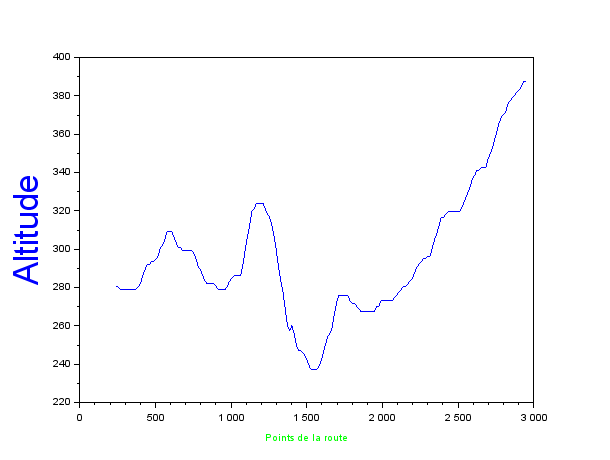
\includegraphics[width=1\linewidth]{0}
\caption{}
\label{fig:0}
\end{figure}

\begin{figure}
\centering
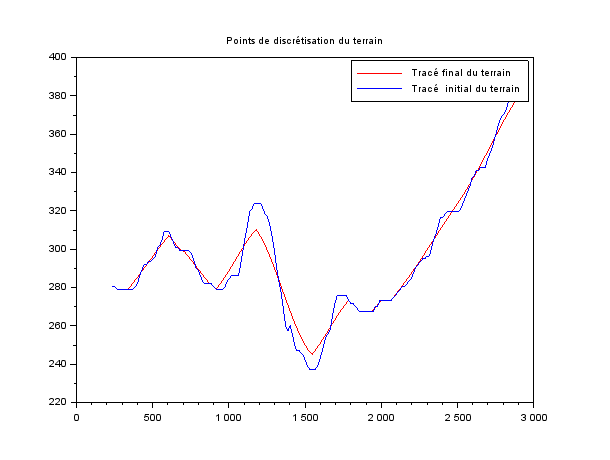
\includegraphics[width=1\linewidth]{1}
\caption{}
\label{fig:1}
\end{figure}

\begin{figure}
	\centering
	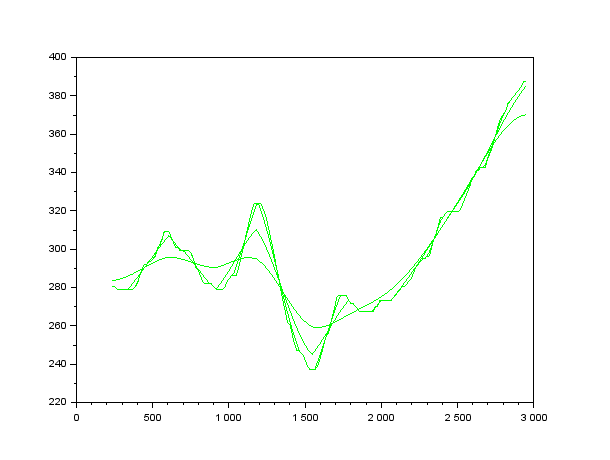
\includegraphics[width=1\linewidth]{2}
	\caption{}
	\label{fig:2}
\end{figure}
\end{document}

